% Provenance (never printed): old seconde/premiere S material on the ocean
% (the ocean as a layered fluid, its heat, upwelling and productive waters);
% see sources/book2/PROVENANCE.md. All profiles are WOA23 columns, all
% densities the EOS-80 one-atmosphere equation, computed in
% figdata/grade-10/ocean_profiles.py.
\chapter{El océano en capas}\label{ch:g10:layered-ocean}

Un día de verano te alejas a nado de una playa, en un agua agradablemente
templada. Dejas colgar las piernas --- y tus pies encuentran un agua de pronto
fría, un par de metros por debajo de la superficie. El mar no está mezclado
de arriba abajo: está hecho de capas, cálidas y ligeras arriba, frías y
densas abajo. En mar abierto, esa misma \omterm{def:g10:layered-ocean:stratification}{estratificación} alcanza kilómetros de
profundidad, y decide dónde el mar es un desierto y dónde rebosa de vida. Este
capítulo mira el océano en profundidad: cómo se mide, cómo cambian hacia abajo
su temperatura y su salinidad, por qué las capas son estables y dónde el agua
fría profunda vuelve a subir a la superficie.

\begin{recall}
El agua de mar contiene sales disueltas: su salinidad, de unos 35 gramos de
sal por kilogramo de agua de mar en promedio, varía de un mar a otro. Los
vientos mueven las corrientes superficiales y los grandes giros oceánicos;
las corrientes profundas de agua fría y salada avanzan lentamente a lo largo
del fondo oceánico (Libro 1, año 8). La densidad es la masa dividida entre el
volumen (los libros de física). El fitoplancton, formado por algas
microscópicas, necesita luz y nutrientes minerales para crecer mediante la
fotosíntesis, y alimenta al resto de las cadenas alimentarias del océano (los
libros de biología).
\end{recall}

\section{Medir el océano}

El océano cubre unos \num{362}~millones de~\unit{km^2} y tiene una profundidad
media de \qty{3682}{m}: unos \num{1.33}~mil millones de~\unit{km^3} de agua. Casi
todo queda muy lejos del alcance de la luz, y solo puede medirse enviando
instrumentos hacia abajo.
% ledger: charette:ocean-volume

Desde un barco, los oceanógrafos bajan con un cable un armazón con sensores
que miden la conductividad del agua (a partir de la cual se calcula su
salinidad), su temperatura y la presión (y, por tanto, la profundidad),
rodeado de un anillo de botellas que se cierran a profundidades elegidas para
subir a bordo muestras de agua. Desde el año 2000, una flota de boyas
robóticas ha añadido millones de perfiles: cada boya deriva con las corrientes
a \qty{1000}{m} de profundidad, se hunde más o menos cada diez días hasta
\qty{2000}{m}, sube luego a la superficie midiendo la temperatura y la
salinidad por el camino, y envía su perfil por satélite.
% ledger: argo:fleet

\begin{dated}{2026}
La red internacional Argo cuenta con cerca de 4000 boyas activas; su perfil
número tres millones se obtuvo en julio de 2024.
% ledger: argo:fleet
\end{dated}

\begin{omfigure}
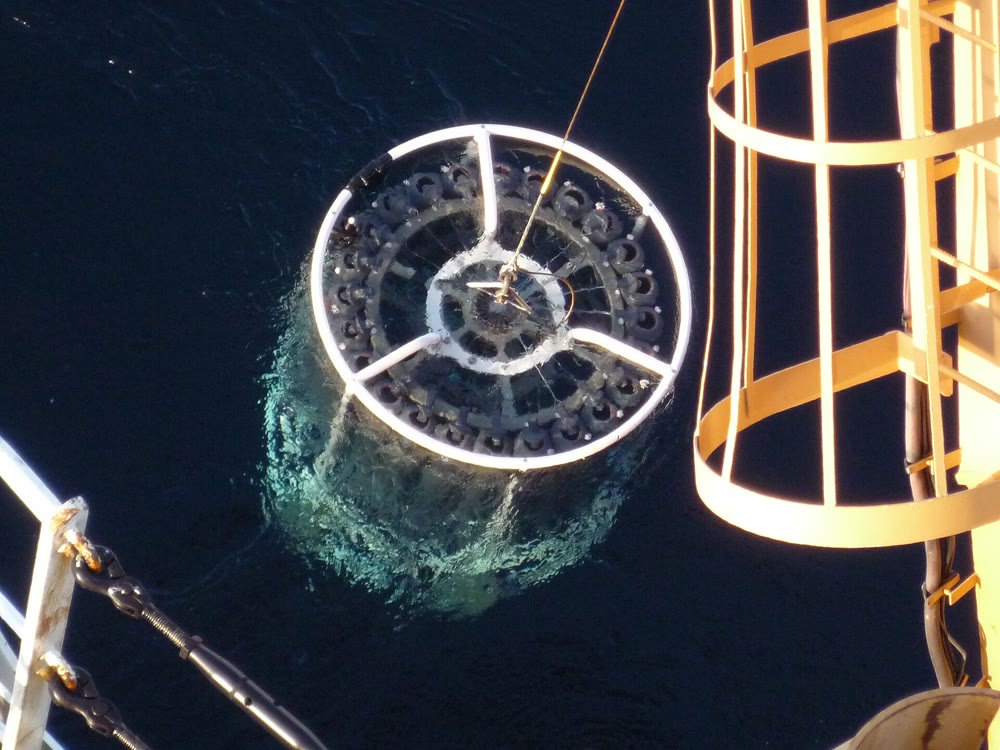
\includegraphics[height=4.4cm]{images/book2/g10-noaa-ctd-rosette.jpg}\hspace{0.4cm}%
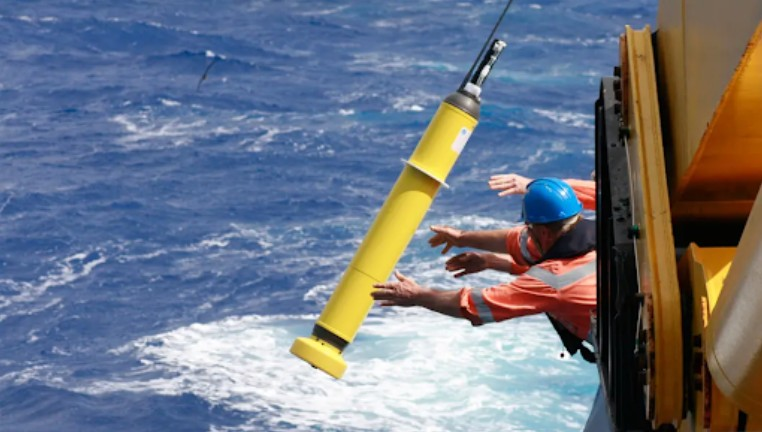
\includegraphics[height=4.4cm]{images/book2/g10-noaa-argo-float.jpg}

{\small Izquierda: una roseta de botellas de muestreo alrededor de sus
sensores, izada junto a un buque oceanográfico en el Ártico, 2008 (fotografía:
Pablo Clemente-Colon, NOAA Photo Library). Derecha: lanzamiento de una boya
perfiladora desde un buque oceanográfico (fotografía: NOAA Global Ocean
Monitoring and Observing Program). Ambas de dominio público.}
\end{omfigure}

Promediados sobre décadas de medidas, estos perfiles dan una imagen del
océano en profundidad. Los perfiles de este capítulo son promedios de este
tipo, tomados del \emph{World Ocean Atlas 2023} de los National Centers for
Environmental Information de la NOAA.

\section{La temperatura en profundidad}

\begin{omfigure}
\begin{tikzpicture}
\begin{axis}[omrecord, omdepth, width=0.62\linewidth, height=8.2cm,
  axis x line=top, xmin=-3, xmax=31, ymin=0, ymax=2000,
  xlabel={temperatura (\unit{\degreeCelsius})}, ylabel={profundidad (\unit{m})},
  tick label style={font=\small}, label style={font=\small},
  legend style={font=\scriptsize, at={(0.98,0.03)}, anchor=south east}]
\addplot[omThm!85!black, thick] table[x=t, y=depth] {figdata/out/grade-10-ocean_profiles-site-warmpool.dat};
\addplot[omDef!85!black, thick] table[x=t, y=depth] {figdata/out/grade-10-ocean_profiles-site-atlantic.dat};
\addplot[black!70, thick, dashed] table[x=t, y=depth] {figdata/out/grade-10-ocean_profiles-site-arctic.dat};
\legend{{Pacífico tropical, 5.5\textdegree N}, {Atlántico Norte, 40.5\textdegree N}, {océano Ártico, 75.5\textdegree N}}
\node[font=\scriptsize, anchor=west] (ml) at (axis cs:21,430) {capa de mezcla};
\draw[black!50] (ml.north east) -- (axis cs:28.9,35);
\node[font=\scriptsize, anchor=west] (tc) at (axis cs:15.5,600) {termoclina};
\draw[black!50] (tc.north) -- (axis cs:19.9,150);
\node[font=\scriptsize, anchor=west] at (axis cs:7,1500) {océano profundo};
\end{axis}
\end{tikzpicture}

{\small Temperatura media en función de la profundidad en tres lugares (la
profundidad aumenta hacia abajo). Datos: World Ocean Atlas 2023, medias
anuales, NOAA NCEI.}
\end{omfigure}
% ledger: data:b2-woa23 (profiles in figdata/grade-10/ocean_profiles.py)

La luz solar calienta el océano desde arriba, en su capa superficial. El viento y el oleaje remueven esta agua cálida hasta formar una capa de
temperatura casi uniforme. Por debajo, la temperatura baja deprisa a lo largo
de unos cientos de metros; más abajo todavía, baja lentamente hasta el agua
fría que llena las cuencas oceánicas.

\begin{definition}[Capa de mezcla]\label{def:g10:layered-ocean:mixed-layer}
La \emph{capa de mezcla}\index{capa de mezcla} es la capa superficial del
océano, removida por el viento y el oleaje, en la que la temperatura y la
salinidad apenas cambian con la profundidad.
\end{definition}

\begin{definition}[Termoclina; haloclina; picnoclina; océano profundo]\label{def:g10:layered-ocean:thermocline}
La \emph{termoclina}\index{termoclina} es la capa situada bajo la \omterm{def:g10:layered-ocean:mixed-layer}{capa de
mezcla} en la que la temperatura baja deprisa con la profundidad. La capa en la
que la salinidad cambia deprisa con la profundidad es una
\emph{haloclina}\index{haloclina}; la capa en la que la densidad aumenta
deprisa con la profundidad es la \emph{picnoclina}\index{picnoclina}. Por
debajo de ellas se extiende el \emph{océano
profundo}\index{oceano profundo@océano profundo}, frío y de cambios lentos.
\end{definition}

En el Pacífico tropical, la \omterm{def:g10:layered-ocean:mixed-layer}{capa de mezcla} está a \qty{29.2}{\degreeCelsius}
y tiene unos \qty{60}{m} de espesor; entre \qty{70}{m} y \qty{300}{m} la
temperatura baja casi diecinueve grados, y a \qty{1000}{m} ya solo es de
\qty{4.5}{\degreeCelsius}. En el Atlántico Norte la superficie es más fresca
y la bajada más gradual. En el océano Ártico, toda la columna se mantiene a
menos de dos grados de \qty{0}{\degreeCelsius}: no hay capa superficial
cálida digna de ese nombre.
% ledger: data:b2-woa23

\begin{method}[Leer un perfil oceánico]\label{met:g10:layered-ocean:profile}
\begin{enumerate}
  \item Identifica los ejes: la profundidad aumenta hacia abajo, y la
        magnitud medida se lee a lo largo del borde superior.
  \item La \omterm{def:g10:layered-ocean:mixed-layer}{capa de mezcla} es la parte superior, donde la curva es casi
        vertical; su profundidad está donde la curva empieza a apartarse de
        la vertical (una regla habitual: donde la temperatura ha bajado
        \qty{0.5}{\degreeCelsius} respecto a su valor en superficie).
  \item La \omterm{def:g10:layered-ocean:thermocline}{termoclina} está donde la curva se acerca más a la horizontal: el
        mayor cambio para la menor profundidad.
  \item Por debajo, lee los valores profundos y compara los lugares a una
        misma profundidad.
\end{enumerate}
\end{method}

La \omterm{def:g10:layered-ocean:mixed-layer}{capa de mezcla} cambia con las estaciones. En invierno la superficie pierde
calor, las tempestades agitan el mar y la \omterm{def:g10:layered-ocean:mixed-layer}{capa de mezcla} se hace más
profunda; en verano el sol calienta una capa superficial delgada que los
vientos, más suaves, no consiguen mezclar hacia abajo, y se forma cerca de la
superficie una \emph{\omterm{def:g10:layered-ocean:thermocline}{termoclina} estacional} --- el agua fría que encuentran
los pies del bañista.

\begin{omfigure}
\begin{tikzpicture}
\begin{axis}[omrecord, omdepth, width=0.6\linewidth, height=6.6cm,
  axis x line=top, xmin=12, xmax=24, ymin=0, ymax=300,
  xlabel={temperatura (\unit{\degreeCelsius})}, ylabel={profundidad (\unit{m})},
  tick label style={font=\small}, label style={font=\small},
  legend style={font=\scriptsize, at={(0.98,0.03)}, anchor=south east}]
\addplot[omDef!85!black, thick] table[x=t_feb, y=depth] {figdata/out/grade-10-ocean_profiles-season.dat};
\addplot[omThm!85!black, thick] table[x=t_aug, y=depth] {figdata/out/grade-10-ocean_profiles-season.dat};
\legend{febrero, agosto}
\end{axis}
\end{tikzpicture}

{\small Invierno y verano en el Atlántico Norte (40.5\textdegree N,
30.5\textdegree O): temperaturas medias mensuales de febrero y de agosto. En
febrero la \omterm{def:g10:layered-ocean:mixed-layer}{capa de mezcla} alcanza unos \qty{170}{m}; en agosto, una capa
cálida de unos \qty{15}{m} de espesor descansa sobre una \omterm{def:g10:layered-ocean:thermocline}{termoclina}
estacional. Datos: World Ocean Atlas 2023, NOAA NCEI.}
\end{omfigure}
% ledger: data:b2-woa23 (mixed-layer depths by the 0.5 degC rule, computed in figdata/grade-10/ocean_profiles.py)

\section{Salinidad y densidad}

La densidad del agua de mar depende de su temperatura y de su salinidad. Se
calcula con una fórmula acordada internacionalmente, la ecuación de estado
del agua de mar, ajustada a medidas de laboratorio.

\begin{proposition}[Densidad del agua de mar]\label{prop:g10:layered-ocean:density}
La densidad del agua de mar aumenta con su salinidad y disminuye cuando sube
su temperatura. A la presión de la superficie, el agua de mar de salinidad 35
tiene una densidad de \qty{1028.1}{kg/m^3} a \qty{0}{\degreeCelsius} y de
\qty{1023.3}{kg/m^3} a \qty{25}{\degreeCelsius}; el agua pura a
\qty{4}{\degreeCelsius} tiene una densidad de \qty{1000.0}{kg/m^3}.
\end{proposition}
% ledger: unesco:eos80 (values computed in figdata/grade-10/ocean_profiles.py)

\begin{omfigure}
\begin{tikzpicture}
\begin{axis}[omrecord, width=0.7\linewidth, height=6.2cm, xmin=-2, xmax=30,
  ymin=1016, ymax=1033, xlabel={temperatura (\unit{\degreeCelsius})},
  ylabel={densidad (\unit{kg/m^3})}, tick label style={font=\small},
  label style={font=\small}, yticklabel style={/pgf/number format/1000 sep={}}]
\addplot[omThm!85!black, thick] table[x=t, y=rho_s38] {figdata/out/grade-10-ocean_profiles-eos.dat};
\addplot[black!80, thick] table[x=t, y=rho_s35] {figdata/out/grade-10-ocean_profiles-eos.dat};
\addplot[omDef!85!black, thick] table[x=t, y=rho_s30] {figdata/out/grade-10-ocean_profiles-eos.dat};
\node[font=\scriptsize, anchor=south west, omThm!85!black] at (axis cs:1,1030.75) {salinidad 38};
\node[font=\scriptsize, anchor=south west] at (axis cs:1,1028.35) {salinidad 35};
\node[font=\scriptsize, anchor=south west, omDef!85!black] at (axis cs:1,1024.35) {salinidad 30};
\end{axis}
\end{tikzpicture}

{\small La densidad del agua de mar a la presión de la superficie, en función
de su temperatura, para tres salinidades (calculada con la ecuación de estado
internacional del agua de mar).}
\end{omfigure}
% ledger: unesco:eos80

En la gráfica se ven dos cosas. Una unidad de salinidad añade unos
\qty{0.8}{kg/m^3}. Un grado de calentamiento quita unos \qty{0.31}{kg/m^3}
a \qty{25}{\degreeCelsius}, \qty{0.18}{kg/m^3} a \qty{10}{\degreeCelsius},
pero solo \qty{0.06}{kg/m^3} cerca de \qty{0}{\degreeCelsius}: en los mares
cálidos la temperatura controla la densidad; en los mares fríos, la salinidad.
% ledger: unesco:eos80 (slopes computed in figdata/grade-10/ocean_profiles.py)

\begin{remark}
Las densidades de este capítulo se calculan a la presión de la superficie.
La presión del agua que hay encima comprime un poco el agua de mar, unos
\qty{4}{kg/m^3} por kilómetro de profundidad; los oceanógrafos comparan las
masas de agua a una misma presión, para que solo cuenten la temperatura y la
salinidad.
\end{remark}
% ledger: unesco:eos80-checks (computed in figdata/grade-10/ocean_profiles.py: 3.9 kg/m3 per km from the 10000-dbar check values)

\begin{omfigure}
\begin{tikzpicture}
\begin{axis}[name=sal, omrecord, omdepth, width=0.5\linewidth, height=7.2cm,
  axis x line=top, xmin=27.5, xmax=37, ymin=0, ymax=1000,
  xlabel={salinidad}, ylabel={profundidad (\unit{m})},
  tick label style={font=\small}, label style={font=\small}]
\addplot[omThm!85!black, thick] table[x=s, y=depth] {figdata/out/grade-10-ocean_profiles-site-warmpool.dat};
\addplot[omDef!85!black, thick] table[x=s, y=depth] {figdata/out/grade-10-ocean_profiles-site-atlantic.dat};
\addplot[black!70, thick, dashed] table[x=s, y=depth] {figdata/out/grade-10-ocean_profiles-site-arctic.dat};
\node[font=\scriptsize, anchor=west, align=left] at (axis cs:28.2,120) {haloclina\\del Ártico};
\end{axis}
\begin{axis}[at={(sal.east)}, anchor=west, xshift=0.9cm, omrecord, omdepth,
  width=0.5\linewidth, height=7.2cm, axis x line=top, xmin=1021, xmax=1028.5, yticklabels={},
  ymin=0, ymax=1000, xlabel={densidad (\unit{kg/m^3})},
  tick label style={font=\small}, label style={font=\small},
  xticklabel style={/pgf/number format/1000 sep={}},
  legend style={font=\scriptsize, at={(0.03,0.03)}, anchor=south west}]
\addplot[omThm!85!black, thick] table[x=rho, y=depth] {figdata/out/grade-10-ocean_profiles-site-warmpool.dat};
\addplot[omDef!85!black, thick] table[x=rho, y=depth] {figdata/out/grade-10-ocean_profiles-site-atlantic.dat};
\addplot[black!70, thick, dashed] table[x=rho, y=depth] {figdata/out/grade-10-ocean_profiles-site-arctic.dat};
\legend{Pacífico tropical, Atlántico Norte, océano Ártico}
\end{axis}
\end{tikzpicture}

{\small Salinidad (izquierda) y densidad a la presión de la superficie
(derecha) en función de la profundidad, en los tres lugares de los perfiles
de temperatura. En todos ellos la densidad aumenta hacia abajo. Datos: World
Ocean Atlas 2023, NOAA NCEI; densidades calculadas con la ecuación de estado
internacional del agua de mar.}
\end{omfigure}
% ledger: data:b2-woa23, unesco:eos80

En el Pacífico tropical, la \omterm{def:g10:layered-ocean:thermocline}{picnoclina} coincide con la \omterm{def:g10:layered-ocean:thermocline}{termoclina}. En el
océano Ártico la temperatura apenas cambia, pero la salinidad sube de 28 en
la superficie, rebajada por los ríos y por el hielo que se funde, a 34.8 a
\qty{500}{m}: la \omterm{def:g10:layered-ocean:thermocline}{haloclina} es la \omterm{def:g10:layered-ocean:thermocline}{picnoclina}. En todos los casos, la densidad
aumenta hacia abajo.
% ledger: data:b2-woa23

\begin{definition}[Estratificación]\label{def:g10:layered-ocean:stratification}
El océano está \emph{estratificado}\index{estratificacion@estratificación}
cuando su densidad aumenta con la profundidad: el agua más ligera descansa
sobre el agua más densa, en capas.
\end{definition}

Un océano \omterm{def:g10:layered-ocean:stratification}{estratificado} es estable. Una porción de agua empujada hacia abajo,
hacia un agua más densa, es más ligera que su entorno y vuelve a flotar hacia
arriba; una porción empujada hacia arriba vuelve a hundirse. Para mezclar las
capas, el viento tiene que trabajar en contra de esto, y cuanto más marcada
es la \omterm{def:g10:layered-ocean:thermocline}{picnoclina}, más difícil resulta: la \omterm{def:g10:layered-ocean:thermocline}{termoclina} es una tapadera que
separa la superficie del \omterm{def:g10:layered-ocean:thermocline}{océano profundo}. El \omterm{def:g10:layered-ocean:thermocline}{océano profundo} está lleno de
agua que se hundió hace mucho tiempo en los mares polares fríos, donde el agua
superficial se vuelve lo bastante densa para hundirse (Libro 1, año 8).

\section{El afloramiento}

\begin{definition}[Afloramiento]\label{def:g10:layered-ocean:upwelling}
El \emph{afloramiento}\index{afloramiento} es la subida de agua fría desde
debajo de la capa superficial, para sustituir al agua superficial que el
viento aparta. Se produce a lo largo de algunas costas y en mar abierto.
\end{definition}
% ledger: noaa:upwelling

A lo largo de una costa, el viento que sopla paralelo a la orilla arrastra el
agua superficial; a causa de la rotación de la Tierra, el agua no sigue sin
más al viento, sino que se desvía de él, hacia la derecha en el hemisferio
norte y hacia la izquierda en el hemisferio sur (cómo ocurre esto es tema de
los volúmenes universitarios). Frente a Perú, el viento sopla a lo largo de la
costa hacia el ecuador, y el agua superficial es empujada mar adentro; cerca
de la costa sube agua fría para ocupar su lugar. También hay \omterm{def:g10:layered-ocean:upwelling}{afloramiento} a
lo largo del ecuador, donde los alisios apartan de él el agua superficial
hacia ambos lados.
% ledger: noaa:upwelling, kessler:peru-upwelling

\begin{omfigure}
\begin{tikzpicture}[font=\footnotesize, >={Stealth[length=2mm]}]
  % ocean and thermocline
  \fill[omDef!12] (0,-3.2) rectangle (8.2,0);
  \fill[omDef!30] (0,-3.2) -- (0,-2.0) .. controls (3,-2.0) and (5.5,-1.6) .. (7.4,-0.35) -- (8.2,0) -- (8.2,-3.2) -- cycle;
  \draw[omDef!80!black, dashed] (0,-2.0) .. controls (3,-2.0) and (5.5,-1.6) .. (7.4,-0.35);
  \node[anchor=north west, omDef!80!black] at (0.1,-2.05) {termoclina};
  \node[anchor=west, black!70] at (0.15,-0.9) {agua superficial cálida};
  \node[anchor=west, black!70] at (0.15,-2.75) {agua fría, rica en nutrientes};
  % land
  \fill[omExo!30, draw=black!60] (7.0,-3.2) -- (8.2,-0.1) -- (8.6,0.0) -- (9.6,1.2) -- (10.6,2.2) -- (10.6,-3.2) -- cycle;
  \node[anchor=south, align=center] at (9.9,-1.6) {tierra};
  % surface flow and rising water
  \draw[->, thick, omThm!80!black] (7.2,-0.3) -- (3.6,-0.3);
  \node[anchor=south, omThm!80!black] at (5.4,-0.25) {agua superficial empujada mar adentro};
  \foreach \x/\y in {6.1/-2.1, 6.8/-1.7} \draw[->, thick, omDef!80!black] (\x,\y) -- (\x+0.45,\y+1.15);
  \node[anchor=north, omDef!80!black, align=center] at (6.0,-2.25) {sube agua fría};
  % wind along the shore, northward: with west on the left and east on the
  % right the reader looks north, so the wind goes into the page
  \draw[black!70, thick] (2.6,1.0) circle (0.22);
  \draw[black!70, thick] (2.6,1.0) ++(45:0.22) -- ++(225:0.44) (2.6,1.0) ++(135:0.22) -- ++(315:0.44);
  \node[anchor=west, align=left] at (2.9,1.0) {viento paralelo a la costa, hacia el ecuador\\(hacia el norte, entrando en la página)};
  \node[anchor=north west, black!60] at (0,-3.25) {$\leftarrow$ oeste};
  \node[anchor=north east, black!60] at (10.6,-3.25) {este $\rightarrow$};
\end{tikzpicture}

{\small \omterm{def:g10:layered-ocean:upwelling}{Afloramiento} costero frente a Perú (corte esquemático de oeste a
este, sin escala): el viento sopla a lo largo de la costa hacia el ecuador,
hacia el norte, entrando en la página; el agua superficial se desvía hacia su
izquierda y es empujada mar adentro; el agua fría de debajo de la \omterm{def:g10:layered-ocean:thermocline}{termoclina}
sube cerca de la costa para sustituirla.}
\end{omfigure}

El agua que sube no solo es fría. Por debajo de la capa superficial
iluminada, los restos del plancton muerto, que se hunden y se descomponen,
liberan los nutrientes minerales que necesita el fitoplancton. Devueltos a la
luz, estos nutrientes hacen de las regiones de \omterm{def:g10:layered-ocean:upwelling}{afloramiento} las aguas más
productivas del océano, con los caladeros más ricos. Donde el océano está muy
\omterm{def:g10:layered-ocean:stratification}{estratificado} y nada sube el agua profunda, la capa iluminada se queda sin
nutrientes: los centros de los giros subtropicales son los desiertos del
océano.
% ledger: noaa:upwelling

\begin{omfigure}
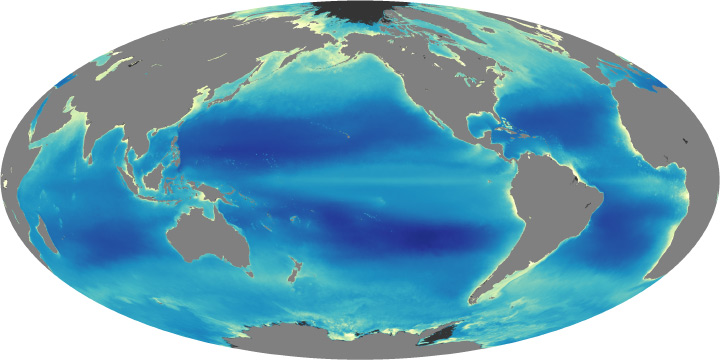
\includegraphics[width=0.8\linewidth]{images/book2/g10-nasa-ocean-chlorophyll.jpg}

{\small La clorofila del fitoplancton vista desde el espacio, promediada
sobre 2002--2010: del azul oscuro (muy poca) al amarillo (mucha), pasando por
el azul claro; las tierras, en gris. Destacan la costa de Perú y la franja a
lo largo del ecuador en el Pacífico; los giros son de un azul profundo.
Imagen: Jesse Allen y Robert Simmon, NASA Earth Observatory (dominio
público).}
\end{omfigure}

\begin{omfigure}
\begin{tikzpicture}
\begin{axis}[omrecord, omdepth, width=0.6\linewidth, height=7.2cm,
  axis x line=top, xmin=4, xmax=26, ymin=0, ymax=600,
  xlabel={temperatura (\unit{\degreeCelsius})}, ylabel={profundidad (\unit{m})},
  tick label style={font=\small}, label style={font=\small},
  legend style={font=\scriptsize, at={(0.98,0.03)}, anchor=south east}]
\addplot[omExo!85!black, thick] table[x=t, y=depth] {figdata/out/grade-10-ocean_profiles-site-peru.dat};
\addplot[omThm!85!black, thick] table[x=t, y=depth] {figdata/out/grade-10-ocean_profiles-site-gyre.dat};
\addplot[black!40, dashed, domain=0:600, samples=2] ({15}, {x});
\legend{{frente a Perú, 13.5\textdegree S}, {giro del Pacífico Sur, 20.5\textdegree S}}
\end{axis}
\end{tikzpicture}

{\small Frente a Perú, el agua fría se acerca a la superficie: el agua a
\qty{15}{\degreeCelsius} (línea discontinua) está a unos \qty{65}{m}, frente
a casi \qty{300}{m} en el centro del giro del Pacífico Sur, que está más
lejos del ecuador. Datos: World Ocean Atlas 2023, medias anuales, NOAA NCEI.}
\end{omfigure}
% ledger: data:b2-woa23

\section{Ejercicios}

\begin{exercise}[$\star$]\label{exo:g10:layered-ocean:1}
Define la \omterm{def:g10:layered-ocean:mixed-layer}{capa de mezcla} y la \omterm{def:g10:layered-ocean:thermocline}{termoclina}. ¿Qué remueve la \omterm{def:g10:layered-ocean:mixed-layer}{capa de mezcla}?
\end{exercise}

\begin{exercise}[$\star$]\label{exo:g10:layered-ocean:2}
Define el \omterm{def:g10:layered-ocean:upwelling}{afloramiento}. ¿Por qué las aguas de las regiones de \omterm{def:g10:layered-ocean:upwelling}{afloramiento}
son ricas en vida?
\end{exercise}

\begin{exercise}[$\star$]\label{exo:g10:layered-ocean:3}
Con los perfiles de temperatura de los tres lugares, da la temperatura en la
superficie y a \qty{1000}{m} en el Pacífico tropical y en el océano Ártico.
\end{exercise}

\begin{exercise}[$\star$]\label{exo:g10:layered-ocean:4}
¿Qué es más denso, el agua de mar de salinidad 35 a \qty{25}{\degreeCelsius}
o a \qty{0}{\degreeCelsius}? ¿El agua de mar de salinidad 35 o el agua pura, a
la misma temperatura? Usa los valores del capítulo.
\end{exercise}

\begin{exercise}[$\star$]\label{exo:g10:layered-ocean:5}
Explica cómo mide una boya perfiladora un perfil del océano, y por qué las
boyas son útiles donde los barcos rara vez llegan.
\end{exercise}

\begin{exercise}[$\star\star$]\label{exo:g10:layered-ocean:6}
El océano cubre \num{361.84}~millones de~\unit{km^2}, con una profundidad
media de \qty{3682}{m}. Calcula su volumen en kilómetros cúbicos. ¿Qué
fracción de su profundidad representan los \qty{100}{m} superiores?
\end{exercise}

\begin{exercise}[$\star\star$]\label{exo:g10:layered-ocean:7}
En el perfil del Atlántico Norte de agosto, la temperatura es de
\qty{22.7}{\degreeCelsius} en la superficie, \qty{22.2}{\degreeCelsius} a
\qty{15}{m}, \qty{21.8}{\degreeCelsius} a \qty{20}{m} y
\qty{17.3}{\degreeCelsius} a \qty{50}{m}. Con la regla del método, estima la
profundidad de la \omterm{def:g10:layered-ocean:mixed-layer}{capa de mezcla}. ¿Cuál es el ritmo medio de bajada de la
temperatura entre \qty{20}{m} y \qty{50}{m}, en grados por metro?
\end{exercise}

\begin{exercise}[$\star\star$]\label{exo:g10:layered-ocean:8}
En ese mismo lugar del Atlántico Norte, la superficie está a
\qty{15.3}{\degreeCelsius} en febrero y a \qty{22.7}{\degreeCelsius} en
agosto, mientras que a \qty{300}{m} está a \qty{13.5}{\degreeCelsius} en los
dos meses. Explica por qué el agua profunda no sigue las estaciones, y por qué
la \omterm{def:g10:layered-ocean:mixed-layer}{capa de mezcla} de invierno es mucho más profunda que la de verano.
\end{exercise}

\begin{exercise}[$\star\star$]\label{exo:g10:layered-ocean:9}
Cerca de \qty{10}{\degreeCelsius}, una unidad de salinidad añade
\qty{0.78}{kg/m^3} a la densidad y un grado de calentamiento quita
\qty{0.18}{kg/m^3}. ¿Cuántos grados de calentamiento compensan una unidad de
salinidad? Responde a la misma pregunta cerca de \qty{0}{\degreeCelsius},
donde un grado solo quita \qty{0.06}{kg/m^3}. ¿Qué concluyes para los mares
polares?
\end{exercise}

\begin{exercise}[$\star\star$]\label{exo:g10:layered-ocean:10}
En el océano Ártico, el agua de la superficie está a
\qty{-1.4}{\degreeCelsius} con una salinidad de 28.1, y a \qty{200}{m} está
a \qty{-1.4}{\degreeCelsius} con una salinidad de 33.3. Sus densidades son
\qty{1022.6}{kg/m^3} y \qty{1026.8}{kg/m^3}. ¿Qué hace más densa el agua
profunda? Nombra la capa que hay entre ellas.
\end{exercise}

\begin{exercise}[$\star\star$]\label{exo:g10:layered-ocean:11}
Explica por qué un océano \omterm{def:g10:layered-ocean:stratification}{estratificado} es estable, con una porción de agua
superficial empujada hacia abajo por una ola.
\end{exercise}

\begin{exercise}[$\star\star\star$]\label{exo:g10:layered-ocean:12}
Un litro de agua de mar de salinidad 35 a \qty{0}{\degreeCelsius} se calienta
hasta \qty{25}{\degreeCelsius}. Con las densidades del capítulo, calcula su
masa y después su nuevo volumen. ¿Cuánto se ha dilatado, en mililitros? Una
capa de océano de \qty{700}{m} de espesor se calienta en la misma proporción:
¿cuánto aumenta su espesor? (Es una enorme exageración del calentamiento real
del océano, usada aquí solo para mostrar el efecto.)
\end{exercise}

\begin{exercise}[$\star\star\star$]\label{exo:g10:layered-ocean:13}
En el Pacífico tropical, la densidad es de \qty{1021.6}{kg/m^3} a
\qty{50}{m} y de \qty{1026.0}{kg/m^3} a \qty{200}{m}; en el Atlántico Norte,
en febrero, la temperatura apenas cambia en los \qty{150}{m} superiores. ¿En
cuál de los dos lugares le costaría menos a una tempestad remover el agua
hasta \qty{150}{m}? Explícalo.
\end{exercise}

\begin{exercise}[$\star\star\star$]\label{exo:g10:layered-ocean:14}
En el mapa de la clorofila, localiza dos regiones de mucha clorofila en mar
abierto, lejos de cualquier costa, y una gran región de muy poca clorofila.
Explica cada una con ayuda del capítulo.
\end{exercise}

\begin{exercise}[$\star\star\star$]\label{exo:g10:layered-ocean:15}
Supón que una boya se hunde de \qty{1000}{m} a \qty{2000}{m} en seis horas, y
luego sube a la superficie en diez horas. Calcula su velocidad vertical media
en cada fase, en centímetros por segundo. Si midiera cada \qty{2}{s} durante
la subida, ¿cuántas medidas tendría un perfil, y qué profundidad separa por
término medio dos de ellas?
\end{exercise}

\section{Problema: un lance de CTD frente a Perú}

\begin{problem}[{Problema de fin de semana --- dos perfiles del Pacífico Sur}]
\label{pb:g10:layered-ocean:1}
% ledger: data:b2-woa23, unesco:eos80 (values rounded from figdata/grade-10/ocean_profiles.py)
La tabla da la temperatura y la salinidad medias, y la densidad calculada a
la presión de la superficie, en dos lugares del Pacífico Sur: frente a Perú
(\qty{13.5}{\degree S}, \qty{77.5}{\degree O}) y en el centro del giro
subtropical (\qty{20.5}{\degree S}, \qty{110.5}{\degree O}).

\begin{center}
\small
\begin{tabular}{c|ccc|ccc}
\hline
 & \multicolumn{3}{c|}{frente a Perú} & \multicolumn{3}{c}{giro} \\
profundidad (\unit{m}) & \unit{\degreeCelsius} & salinidad & \unit{kg/m^3} & \unit{\degreeCelsius} & salinidad & \unit{kg/m^3} \\
\hline
0 & 19.0 & 35.08 & 1025.08 & 24.0 & 36.41 & 1024.71 \\
25 & 17.4 & 35.06 & 1025.47 & 23.9 & 36.39 & 1024.73 \\
50 & 15.8 & 35.03 & 1025.83 & 23.6 & 36.38 & 1024.80 \\
100 & 13.7 & 34.93 & 1026.20 & 22.6 & 36.27 & 1025.02 \\
200 & 12.4 & 34.89 & 1026.44 & 20.3 & 35.80 & 1025.30 \\
300 & 11.1 & 34.80 & 1026.62 & 14.4 & 34.76 & 1025.92 \\
500 & 7.9 & 34.60 & 1026.97 & 7.1 & 34.39 & 1026.92 \\
\hline
\end{tabular}
\end{center}

\medskip
\noindent\textbf{Parte I --- Leer los perfiles.}
\begin{enumerate}
  \item ¿Qué lugar es más cálido en la superficie, y por cuánto?
  \item ¿Qué lugar está más lejos del ecuador? ¿Es la diferencia de
        temperatura en superficie la que cabría esperar solo por las
        latitudes?
  \item Con la regla del método, estima la profundidad de la \omterm{def:g10:layered-ocean:mixed-layer}{capa de mezcla}
        en el giro.
  \item ¿Hay \omterm{def:g10:layered-ocean:mixed-layer}{capa de mezcla} frente a Perú? Describe los \qty{100}{m}
        superiores.
  \item ¿Entre qué profundidades baja más deprisa la temperatura en el giro?
        Da el ritmo, en grados por cada cien metros.
  \item ¿A qué profundidad, aproximadamente, está el agua a
        \qty{15}{\degreeCelsius} en cada lugar?
\end{enumerate}

\medskip
\noindent\textbf{Parte II --- Densidades.}
\begin{enumerate}[resume]
  \item Comprueba que la densidad aumenta con la profundidad en los dos
        lugares. ¿Qué te dice esto sobre su estabilidad?
  \item En el giro, el agua superficial es más salada que frente a Perú.
        ¿Debería eso hacerla más densa o más ligera? ¿Es más densa?
  \item Explica cuál de los dos efectos se impone.
  \item Calcula el aumento de densidad desde la superficie hasta
        \qty{200}{m} frente a Perú.
  \item Calcula el mismo aumento en el giro.
\end{enumerate}

\medskip
\noindent\textbf{Parte III --- Comparar la estratificación.}
\begin{enumerate}[resume]
  \item En el giro, ¿dónde se encuentra la mayor parte del aumento de
        densidad de los \qty{500}{m} superiores: por encima o por debajo de
        \qty{200}{m}?
  \item ¿Y frente a Perú?
  \item A \qty{500}{m}, compara los dos lugares. ¿Qué sugiere esto sobre el
        agua profunda que hay debajo de ambos?
  \item Explica en unas pocas frases cómo se ha levantado la \omterm{def:g10:layered-ocean:thermocline}{termoclina}
        frente a Perú hacia la superficie.
  \item El fitoplancton vive en las primeras decenas de metros. ¿En qué lugar
        está el agua rica en nutrientes de debajo de la \omterm{def:g10:layered-ocean:thermocline}{termoclina} al alcance
        de la mezcla producida por el viento? Explícalo.
\end{enumerate}

\medskip
\noindent\textbf{Parte IV --- Por qué son productivas las aguas peruanas.}
\begin{enumerate}[resume]
  \item ¿Cómo sería el agua superficial frente a Perú si el viento paralelo
        a la costa dejara de soplar durante meses?
  \item Con el mapa de la clorofila, compara los dos lugares.
  \item Explica por qué se dice que el giro es un desierto del océano aunque
        esté lleno de luz solar.
  \item Calcula el cociente de los aumentos de densidad desde la superficie
        hasta \qty{200}{m} frente a Perú y en el giro, y di qué muestra.
\end{enumerate}
\end{problem}
